% Options for packages loaded elsewhere
\PassOptionsToPackage{unicode}{hyperref}
\PassOptionsToPackage{hyphens}{url}
%
\documentclass[
]{book}
\usepackage{lmodern}
\usepackage{amssymb,amsmath}
\usepackage{ifxetex,ifluatex}
\ifnum 0\ifxetex 1\fi\ifluatex 1\fi=0 % if pdftex
  \usepackage[T1]{fontenc}
  \usepackage[utf8]{inputenc}
  \usepackage{textcomp} % provide euro and other symbols
\else % if luatex or xetex
  \usepackage{unicode-math}
  \defaultfontfeatures{Scale=MatchLowercase}
  \defaultfontfeatures[\rmfamily]{Ligatures=TeX,Scale=1}
\fi
% Use upquote if available, for straight quotes in verbatim environments
\IfFileExists{upquote.sty}{\usepackage{upquote}}{}
\IfFileExists{microtype.sty}{% use microtype if available
  \usepackage[]{microtype}
  \UseMicrotypeSet[protrusion]{basicmath} % disable protrusion for tt fonts
}{}
\makeatletter
\@ifundefined{KOMAClassName}{% if non-KOMA class
  \IfFileExists{parskip.sty}{%
    \usepackage{parskip}
  }{% else
    \setlength{\parindent}{0pt}
    \setlength{\parskip}{6pt plus 2pt minus 1pt}}
}{% if KOMA class
  \KOMAoptions{parskip=half}}
\makeatother
\usepackage{xcolor}
\IfFileExists{xurl.sty}{\usepackage{xurl}}{} % add URL line breaks if available
\IfFileExists{bookmark.sty}{\usepackage{bookmark}}{\usepackage{hyperref}}
\hypersetup{
  pdftitle={Statistics with R},
  pdfauthor={Krisna Gupta; Donny Pasaribu},
  hidelinks,
  pdfcreator={LaTeX via pandoc}}
\urlstyle{same} % disable monospaced font for URLs
\usepackage{color}
\usepackage{fancyvrb}
\newcommand{\VerbBar}{|}
\newcommand{\VERB}{\Verb[commandchars=\\\{\}]}
\DefineVerbatimEnvironment{Highlighting}{Verbatim}{commandchars=\\\{\}}
% Add ',fontsize=\small' for more characters per line
\usepackage{framed}
\definecolor{shadecolor}{RGB}{248,248,248}
\newenvironment{Shaded}{\begin{snugshade}}{\end{snugshade}}
\newcommand{\AlertTok}[1]{\textcolor[rgb]{0.94,0.16,0.16}{#1}}
\newcommand{\AnnotationTok}[1]{\textcolor[rgb]{0.56,0.35,0.01}{\textbf{\textit{#1}}}}
\newcommand{\AttributeTok}[1]{\textcolor[rgb]{0.77,0.63,0.00}{#1}}
\newcommand{\BaseNTok}[1]{\textcolor[rgb]{0.00,0.00,0.81}{#1}}
\newcommand{\BuiltInTok}[1]{#1}
\newcommand{\CharTok}[1]{\textcolor[rgb]{0.31,0.60,0.02}{#1}}
\newcommand{\CommentTok}[1]{\textcolor[rgb]{0.56,0.35,0.01}{\textit{#1}}}
\newcommand{\CommentVarTok}[1]{\textcolor[rgb]{0.56,0.35,0.01}{\textbf{\textit{#1}}}}
\newcommand{\ConstantTok}[1]{\textcolor[rgb]{0.00,0.00,0.00}{#1}}
\newcommand{\ControlFlowTok}[1]{\textcolor[rgb]{0.13,0.29,0.53}{\textbf{#1}}}
\newcommand{\DataTypeTok}[1]{\textcolor[rgb]{0.13,0.29,0.53}{#1}}
\newcommand{\DecValTok}[1]{\textcolor[rgb]{0.00,0.00,0.81}{#1}}
\newcommand{\DocumentationTok}[1]{\textcolor[rgb]{0.56,0.35,0.01}{\textbf{\textit{#1}}}}
\newcommand{\ErrorTok}[1]{\textcolor[rgb]{0.64,0.00,0.00}{\textbf{#1}}}
\newcommand{\ExtensionTok}[1]{#1}
\newcommand{\FloatTok}[1]{\textcolor[rgb]{0.00,0.00,0.81}{#1}}
\newcommand{\FunctionTok}[1]{\textcolor[rgb]{0.00,0.00,0.00}{#1}}
\newcommand{\ImportTok}[1]{#1}
\newcommand{\InformationTok}[1]{\textcolor[rgb]{0.56,0.35,0.01}{\textbf{\textit{#1}}}}
\newcommand{\KeywordTok}[1]{\textcolor[rgb]{0.13,0.29,0.53}{\textbf{#1}}}
\newcommand{\NormalTok}[1]{#1}
\newcommand{\OperatorTok}[1]{\textcolor[rgb]{0.81,0.36,0.00}{\textbf{#1}}}
\newcommand{\OtherTok}[1]{\textcolor[rgb]{0.56,0.35,0.01}{#1}}
\newcommand{\PreprocessorTok}[1]{\textcolor[rgb]{0.56,0.35,0.01}{\textit{#1}}}
\newcommand{\RegionMarkerTok}[1]{#1}
\newcommand{\SpecialCharTok}[1]{\textcolor[rgb]{0.00,0.00,0.00}{#1}}
\newcommand{\SpecialStringTok}[1]{\textcolor[rgb]{0.31,0.60,0.02}{#1}}
\newcommand{\StringTok}[1]{\textcolor[rgb]{0.31,0.60,0.02}{#1}}
\newcommand{\VariableTok}[1]{\textcolor[rgb]{0.00,0.00,0.00}{#1}}
\newcommand{\VerbatimStringTok}[1]{\textcolor[rgb]{0.31,0.60,0.02}{#1}}
\newcommand{\WarningTok}[1]{\textcolor[rgb]{0.56,0.35,0.01}{\textbf{\textit{#1}}}}
\usepackage{longtable,booktabs}
% Correct order of tables after \paragraph or \subparagraph
\usepackage{etoolbox}
\makeatletter
\patchcmd\longtable{\par}{\if@noskipsec\mbox{}\fi\par}{}{}
\makeatother
% Allow footnotes in longtable head/foot
\IfFileExists{footnotehyper.sty}{\usepackage{footnotehyper}}{\usepackage{footnote}}
\makesavenoteenv{longtable}
\usepackage{graphicx,grffile}
\makeatletter
\def\maxwidth{\ifdim\Gin@nat@width>\linewidth\linewidth\else\Gin@nat@width\fi}
\def\maxheight{\ifdim\Gin@nat@height>\textheight\textheight\else\Gin@nat@height\fi}
\makeatother
% Scale images if necessary, so that they will not overflow the page
% margins by default, and it is still possible to overwrite the defaults
% using explicit options in \includegraphics[width, height, ...]{}
\setkeys{Gin}{width=\maxwidth,height=\maxheight,keepaspectratio}
% Set default figure placement to htbp
\makeatletter
\def\fps@figure{htbp}
\makeatother
\setlength{\emergencystretch}{3em} % prevent overfull lines
\providecommand{\tightlist}{%
  \setlength{\itemsep}{0pt}\setlength{\parskip}{0pt}}
\setcounter{secnumdepth}{5}
\usepackage{booktabs}
\usepackage{amsthm}
\makeatletter
\def\thm@space@setup{%
  \thm@preskip=8pt plus 2pt minus 4pt
  \thm@postskip=\thm@preskip
}
\makeatother
\usepackage[]{natbib}
\bibliographystyle{apalike}

\title{Statistics with R}
\author{Krisna Gupta\footnote{\href{mailto:krisna.gupta@anu.edu.au}{\nolinkurl{krisna.gupta@anu.edu.au}}} \and Donny Pasaribu}
\date{2020-08-10}

\begin{document}
\maketitle

{
\setcounter{tocdepth}{1}
\tableofcontents
}
\hypertarget{some-introduction}{%
\chapter{Some Introduction}\label{some-introduction}}

🚧 Under Construction 🚧

\hypertarget{about-this-book}{%
\section{About this book}\label{about-this-book}}

\hypertarget{what-is-this-book-and-why}{%
\subsection{What is this book and why}\label{what-is-this-book-and-why}}

\hypertarget{learning-outcome}{%
\subsection{Learning outcome}\label{learning-outcome}}

Information in this book would help you to:

\begin{itemize}
\tightlist
\item
  install and update R and Rstudio with ease
\item
  input, edit, and manage dataset
\item
  visualise dataset as needed
\item
  conducting hypothesis testing
\item
  running a regression
\item
  write a report using the results from above
\end{itemize}

\hypertarget{pre-requisite}{%
\subsection{Pre-requisite}\label{pre-requisite}}

This book is intended to anyone who are interested in learning statistics using R language. It is assumed that people has zero experience with using any programing language at all. Experience with spreadsheet program such as Microsoft Excel or Google Sheet is certainly helpful but not needed.

This book will not cover a lot of the theoretical part of statistics. Readers are assumed to understand that already. A little bit of intro will be given but that is pretty much it. Readers are expected to understand already the theory behind these techniques, or are expected to learn it from elsewhere.

\hypertarget{about-r}{%
\section{About R}\label{about-r}}

\hypertarget{what-is-r}{%
\subsection{What is R}\label{what-is-r}}

\hypertarget{good-reasons-to-start-with-r}{%
\subsection{Good reasons to start with R}\label{good-reasons-to-start-with-r}}

\hypertarget{popular}{%
\subsubsection{popular}\label{popular}}

\hypertarget{easy-to-learn}{%
\subsubsection{easy to learn}\label{easy-to-learn}}

\hypertarget{open-source}{%
\subsubsection{open source}\label{open-source}}

\hypertarget{computer-requirements}{%
\subsection{Computer requirements}\label{computer-requirements}}

\hypertarget{what-the-hell-is-r}{%
\chapter{What the hell is R?}\label{what-the-hell-is-r}}

🚧 Under Construction 🚧

This chapter contains instruction

\hypertarget{installing-r-and-rstudio}{%
\section{Installing R and RStudio}\label{installing-r-and-rstudio}}

\hypertarget{rstudios-interface}{%
\section{RStudio's interface}\label{rstudios-interface}}

RStudio looks like this:
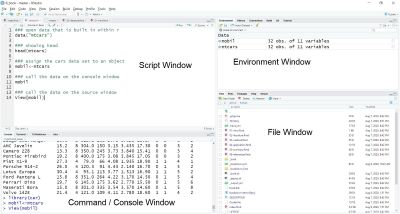
\includegraphics{tampilanR2.JPG}
As you can see from the above figure, RStudio have four main windows.

\hypertarget{console-window}{%
\subsection{console window}\label{console-window}}

Arguably the most important window in RStudio. We write R command in this window.

\hypertarget{script-window}{%
\subsection{script window}\label{script-window}}

Forget what we said about the previous window. This is the most important window in RStudio. We write our sets of command in this window

\hypertarget{environment-window}{%
\subsection{environment window}\label{environment-window}}

You can observe your environment here, such as the data and variables / series you created. This window also have other useful tab such as ``history'' which can show you the history of what happens in your environment, but we will skip them for now.

\hypertarget{files-window}{%
\subsection{files window}\label{files-window}}

Although we call it `files window', this window consists of 5 tabs. The tab file shows your working directory. When you run a code that generates file such as graphics, it will be stored in this window. Plots tab shows you your latest plot.

Packages tab show you all the package that you have. You can also add new package from this tab instead of using the \texttt{install.packages()} command. In this tab, you can also activate package that you have instead of using \texttt{library()} command.

``help'' tab will show you some information about things that you ask help for when you use \texttt{?\textquotesingle{}command\textquotesingle{}} command. Will show you how it works in a minute.

Lastly, ``viewer'' tab. I actually forgot why it exists so whatever.

\hypertarget{using-your-console-window}{%
\section{using your console window}\label{using-your-console-window}}

\hypertarget{using-rscript}{%
\section{using Rscript}\label{using-rscript}}

\hypertarget{package}{%
\section{package}\label{package}}

\hypertarget{update}{%
\section{Update}\label{update}}

You need to keep your R, RStudio and your installed packages updated as much as you can.

\hypertarget{beginner-stuff}{%
\chapter{Beginner stuff}\label{beginner-stuff}}

🚧 Under Construction 🚧

This chapter contains instruction the most basic and useful commands in R. We also covers data types and why it matters.

\hypertarget{setting-your-preamble}{%
\section{Setting your preamble}\label{setting-your-preamble}}

Firstly, it is a good idea to start your script with a clearing environment sets of code.

\begin{Shaded}
\begin{Highlighting}[]
\CommentTok{# Close all graphics, clear memory and screen}
\KeywordTok{graphics.off}\NormalTok{(); }\KeywordTok{remove}\NormalTok{(}\DataTypeTok{list=}\KeywordTok{ls}\NormalTok{());}\KeywordTok{cat}\NormalTok{(}\StringTok{"\textbackslash{}14"}\NormalTok{);}
\end{Highlighting}
\end{Shaded}

There are three different command in this script. \texttt{graphics.off()} clears out the environment from any graphs from previous R session. the command \texttt{remove(list=ls())} is used to remove your environment from any data and variables/series that you may have. Lastly, \texttt{cat("\textbackslash{}14")} clears your console window.

You need to set your working directory

\begin{Shaded}
\begin{Highlighting}[]
\KeywordTok{setwd}\NormalTok{(}\StringTok{'your directory'}\NormalTok{)}
\end{Highlighting}
\end{Shaded}

\hypertarget{data-management}{%
\chapter{Data Management}\label{data-management}}

🚧 Under Construction 🚧

\hypertarget{inferences}{%
\chapter{Inferences}\label{inferences}}

🚧 Under Construction 🚧

\texttt{mean(price)}
\texttt{summary(price)}
\texttt{var(price)}
\texttt{sd(price)}
\texttt{cov(price,\ bedrooms)}
\texttt{cor(price,\ bedrooms)}

\hypertarget{visualisation}{%
\chapter{Visualisation}\label{visualisation}}

🚧 Under Construction 🚧

\hypertarget{plot-command}{%
\section{Plot command}\label{plot-command}}

\texttt{plot()} have many options in it

\hypertarget{using-ggplot2}{%
\section{using ggplot2}\label{using-ggplot2}}

\hypertarget{hypothesis-testing}{%
\chapter{Hypothesis Testing}\label{hypothesis-testing}}

🚧 Under Construction 🚧

\hypertarget{simple-regression}{%
\chapter{Simple Regression}\label{simple-regression}}

🚧 Under Construction 🚧

\hypertarget{univariate-regression}{%
\section{Univariate regression}\label{univariate-regression}}

\hypertarget{plotting-your-regression}{%
\section{plotting your regression}\label{plotting-your-regression}}

In the previous chapter, we have learned how to plot our data using \texttt{plot()}. You can add to your script a line showing your regression result

\hypertarget{multivariate-regression}{%
\section{Multivariate regression}\label{multivariate-regression}}

  \bibliography{book.bib,packages.bib}

\end{document}
